\documentclass{article}

\usepackage[T1]{fontenc}
\usepackage{graphicx}
\usepackage[utf8]{inputenc}

\title{Laboratorium 1 - Analiza błędów}
\author{Mateusz Król}
\date{06/03/2024 r.}

\begin{document}
\maketitle


\section*{Zadanie 1}
\textbf{Oblicz przybliżoną wartość pochodnej funkcji tan(x) dla x = 1.} 
\newline\newline
Dla wzoru $f'(x)\approx\frac{f(x+h)-f(x)}{h}$, błędy prezentują się następująco:
\begin{figure}[h!]
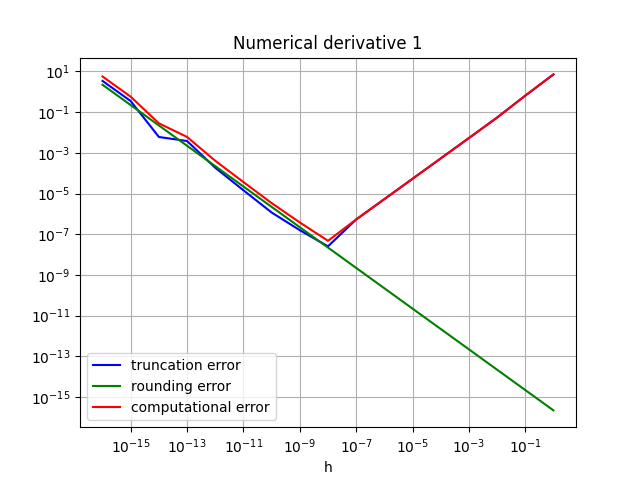
\includegraphics[width=\linewidth]{figures/numerical_derivative_1.png}
\end{figure}
\newline
Wyznaczona wartość: $h_{min} = 10^{-8}$ \newline
Wartość otrzymana ze wzoru $h_{min} \approx 2\cdot\sqrt[]{\epsilon/M}$,
gdzie $M \approx \left|f''(x)\right|$: \newline
$$M\approx \left|\frac{2 \cdot sin(x)}{cos^{3}(x)}\right|
\approx \left|\frac{2 \cdot sin(1)}{cos^{3}(1)}\right|
\approx 10.67$$

$$h_{min} \approx 2\cdot\sqrt[]{2^{-53}/10.67}
\approx 6.45 \cdot 10^{-9}$$

Otrzymane wartości są tego samego rzędu wielkości.  \newline

Dla wzoru $f'(x)\approx\frac{f(x+h)-f(x-h)}{2h}$, błędy prezentują się następująco:
\begin{figure}[h!]
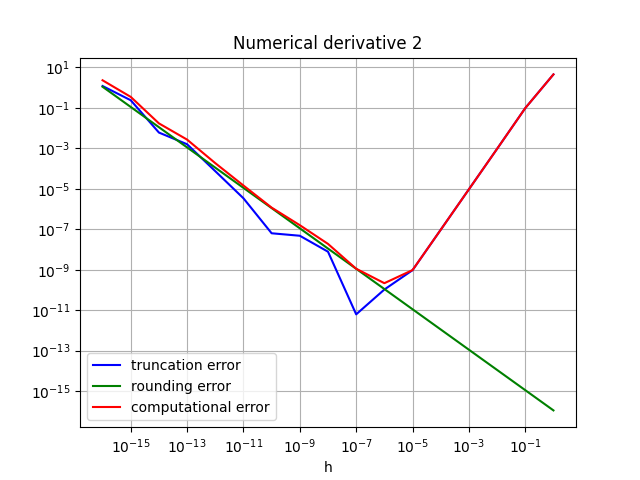
\includegraphics[width=\linewidth]{figures/numerical_derivative_2.png}
\end{figure}
\newline
Wyznaczona wartość: $h_{min} = 10^{-6}$ \newline
Wartość otrzymana ze wzoru $h_{min} \approx \sqrt[3]{3\cdot\epsilon/M}$,
gdzie $M \approx \left|f'''(x)\right|$: \newline
$$M\approx \left|\frac{32\cdot cos^4(x)}{(1 + cos(2 x))^4} + \frac{16\cdot cos^2(x)\cdot sin^2(2 x)}{(1 + cos(2 x))^4}\right|
\approx 56.7$$

$$h_{min} \approx \sqrt[3]{3\cdot2^{-53}/56.7}
\approx 1.8 \cdot 10^{-6}$$

Otrzymane wartości są tego samego rzędu wielkości.  \newline

\section*{Zadanie 2}
\textbf{Napisz program generujący pierwsze n wyrazów ciągu zdefiniowa-
nego równaniem różnicowym:}
$$x_{k+1} = 2.25\cdot x_k - 0.5\cdot x_{k-1}$$, gdzie $x_0 = \frac{1}{3}$, $ x_1 = \frac{1}{12}$.
\newline\newline








\end{document}